\documentclass{thesis}%
\usepackage[T1]{fontenc}%
\usepackage[utf8]{inputenc}%
\usepackage{lmodern}%
\usepackage{textcomp}%
\usepackage{lastpage}%
\usepackage{graphicx}%
\usepackage{caption}%
\usepackage{indentfirst}%
\usepackage{titlesec}%
\usepackage{amsfonts}%
\usepackage{amsmath}%
\usepackage{subfigure}%
\usepackage[none]{hyphenat}%žádné dělení slov

\begin{document}%
\section{B-Spline registrace}

\begin{equation}
v(x)=\sum_i p_i \beta_i(x)
\end{equation}

\begin{equation}
\Sigma = \{(x,y,z)|0 \leq x \leq X, 0 \leq y \leq Y, 0 \leq z \leq Z \}
\end{equation}
Nyní definujme síť kontrolních bodů $\Psi$ s rozměry $n_x x n_y x n_z$. Pro body $\Psi_{i,j,k}$ můžeme zapsat:
\begin{equation}
T_{nonrigid}(x,y,z)= \sum_{i=0}^3\sum_{m=0}^3\sum_{n=0}^3 B_i(u)B_m(v)B_n(w) \Psi_{l, m, n} 
\end{equation}
kde $B_x, x\in(i,j,k)$ jsou bázové funkce a $\Psi$ reprezentuje deformační mřížku. Pro registaci obrazových dat v lékařství se nejčastěji používá jako řídící oblast osmiokolí bodu. Vzdálenosti je pak definována následovně:
\begin{equation}
\Omega_x = [\frac{x}{N_x}]-1,\\
\Omega_y = [\frac{y}{N_y}]-1,\\
\Omega_z = [\frac{z}{N_z}]-1
\end{equation}
kde $N$ je počet voxelů pro osy $x,y$ a $z$. Posun každého voxelu v okolí $\Omega(x,y,z)$ je ovlivněn zhruba 64 kontrolními body. Souřadnice 64 kontrolních bodů $CP(l,m,n)$ vypočteme následujicím způsobem:
\begin{equation}
CP_l = [\frac{x}{N_x}-1+i],\\
CP_m = [\frac{y}{N_y}-1+j],\\
CP_n = [\frac{z}{N_z}-1+k]
\end{equation}
Jednotlivé lokální souřadnice $Local(u,v,w)$ v oblasti $\Omega(x,y,z)$ a hodnota je normalizována do intervalu $[0,1]$. Poté je možné zapsat
\begin{equation}
Local_u =\frac{x}{N_x}-[\frac{x}{N_x}],\\
Local_v =\frac{y}{N_y}-[\frac{y}{N_y}],\\
Local_w =\frac{z}{N_z}-[\frac{z}{N_z}]
\end{equation}
\section{Metoda založená na vlastních číslech Hessovi matice - Frangiho filtr}
Hessova matice je maticí druhých parciálních derivací skalární funkce a má následující tvar:

\begin{equation}
H(f) = \left| \begin{array}{cccc}
\frac{\partial^2 f}{\partial x_{1}^2} & \frac{\partial^2 f}{\partial x_1 \partial x_2} & ... &  \frac{\partial^2 f}{\partial x_1 \partial x_n}\\
\frac{\partial^2 f}{\partial x_2\partial x_1} & \frac{\partial^2 f}{\partial x_2^2} & ... &  \frac{\partial^2 f}{\partial x_2 \partial x_n}\\
... & ... & ... & ...\\
\frac{\partial^2 f}{\partial x_n \partial x_1} & \frac{\partial^2 f}{\partial x_n \partial x_2} & ... &  \frac{\partial^2 f}{\partial x_n^2}
\end{array} \right|
\end{equation}
Frangiho segmentační filtr pracuje s faktem, že cévy jsou válcovité struktury. Pro každý jeden voxel tedy zkoumá okolí a takovéto struktury hledá.\\ V problematice segmentace je možné použít \\\
Hessovu matici použivá jako konvoluční filtr. Následně provedeme dekompozici na vlastní vektory. Vzhledem k tomu, že je použita matice 3x3 dostaneme pro každý voxel obrazu tři vlastní vektory. Tato sada vektorů reprezentuje zkoumaný voxel v novém ortonormálním souřadnicovém systému a obsahuje infomraci o zakřivení zkoumaného obrazu. Vlastní čísla kvantifikují velikost zakřivení v jednotlivých směrem a je tedy možné je použít pro hledání různých typů struktur (viz tabulka XX). Díky tomuz je možné najít cévám podobné obrazy na základě zkoumání vlastních vektorů Hessovy matice.\\
Mějme tedy vlastní čísla $\lambda_1 \leq \lambda_1 \leq \lambda_1$ cévy nebo obecněji válcovité struktury pak v odpovídají myšlence, že ve dvou směrech je zakřivení velké a ve třetím směru naopak malé. tj.:

\begin{equation}
|\lambda_1| \approx 0, |\lambda_1|\ll |\lambda_2|, |\lambda_3|
\end{equation}
Pro usnadnění klasifikace jednotlivých struktur je ve Frangiho filtru definováno několik poměrů například:
 \begin{equation}
R_A = \frac{|\lambda_2|}{|\lambda_3|}
\end{equation}
, který rozlišuje válcovitých od dekovitých struktur. Jak bylo zminěno výše $ \lambda_2$ a $\lambda_3$ jsou v případě cév téměř stejně velké a hodnota $\lambda_1$ je naopak malá po celé délce struktury. Pokud se jedná plochou deskovitou strukturu jesou první dvě hodnoty malé (tj. $\lambda_1$ a $\lambda_2$) a pouze hodnota $\lambda_3$ je výrazně vyšší. Pokud se tedy jedná o válcovitou cévám podobnou strukturu, blíží se poměr $R_A$ hodnotě $1$. Naopak pokud bude hodnota tohoto poměru v blízkosti $0$, jedná se o plochou strukturu.\\
Definujme dále poměr $R_B$: 
 \begin{equation}
R_B = \frac{|\lambda_1|}{\sqrt{|\lambda_2||\lambda_3|}}
\end{equation}
, díky němuž je možné oddělit válcovité a kulovité struktury. Kulovité struktury mají vlastní čísla Hessovi matice zhruba stejně velká. $R_B$ tedy dosahuje svého maxima blížícího se 1 právě pro kulovité struktury, zatímco pro ostatní hodnotu blížící se 0.\\
Další informaci o struktuře a tvaru můžeme získat z tzv. \textit{Frangi's structureness measure} (v češtine možno říci Frangiho míru strukturality):
 \begin{equation}
S = ||H||_F = \sqrt{\sum_{j\leq D}\lambda^2} = \sqrt{\sum \lambda_1^2 + \lambda_2^2 + \lambda_3^2}
\end{equation}
Tato míra je Frobeniovou normou matice a díky ní můžeme oddělit šum a strukturu nebo oblast zájmu. Frobeniova norma uvažuje velikost všech tří vlastních čísel z nichž pro libovolnou strukturu bude minimálně jedno obsahovat vysokou hodnotu narozdíl od šumu. \\
Frangiho celková míra podobnosti cévní struktuře je pak spočítána následujícím způsobem:
 \begin{equation}\label{Frangiho celková míra}
V(x,s) = \Big\{   \begin{array}{c}
0 \;\;\;\;\;\;\;\;\;\;\;\;\;\;\;\;\;\;\;\;\;\;\;\;\;\;\;\;\;\;\;\;\;\;pokud\; \lambda_2 > 0 \;nebo\; \lambda_3 > 0\\
(1-exp(\frac{-R_A^2}{2\alpha^2}))exp(\frac{-R_B^2}{2\beta^2})(1-exp(\frac{-S^2}{2 \gamma^2}))\;\;\;\;\;jinak
\end{array}\end{equation}
Kde $\alpha,\beta$ a $\gamma$ jsou prahové hodnoty definující citlivost Frangiho na jednotlivé typy struktur a šum. Dle definice Frangiho míry  \ref{Frangiho celková míra} jsou také zanedbány voxely, pro něž jsou vlastní čísla matice $\lambda_2$ a $\lambda_3$ větší než 0. Právě tato vlastnost indikuje, že se jedná o voxely s nízkou optickou absorbcí na pozadí. Pro přehlednost je význam jednotlivých vlastních čísel Hessovy matice uveden v následující tabulce:
\begin{center} 
\begin{tabular}{c c c c c}
\hline
$\lambda_1$ & $\lambda_2$  & $\lambda_3$ & Tvar struktury& \\
\hline
malé & velké  & velké & válcovitá &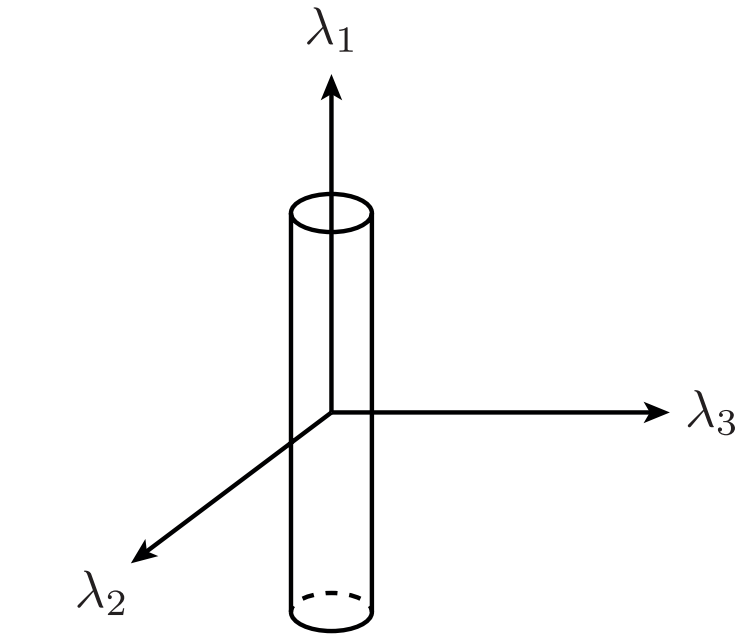
\includegraphics[width=1.2cm]{imgs/tube.png} \\
\hline
malé & malé  & velké & plochá, talířovitá &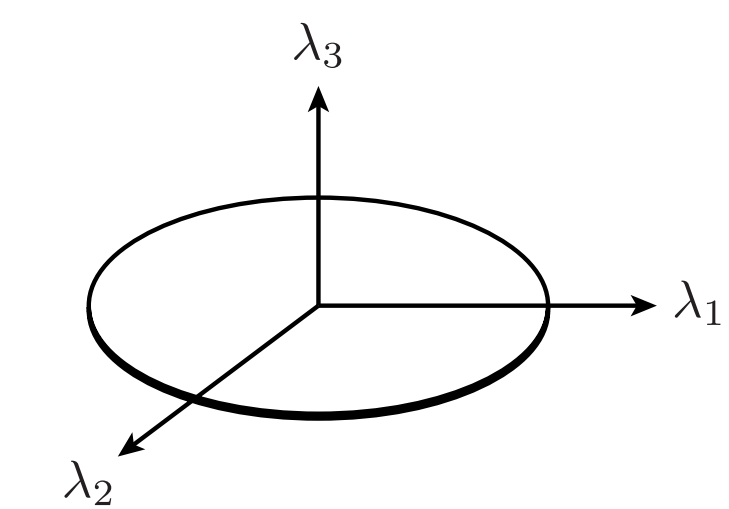
\includegraphics[width=1.2cm]{imgs/plate.png} \\
\hline
velké & velké  & velké & kulovitá &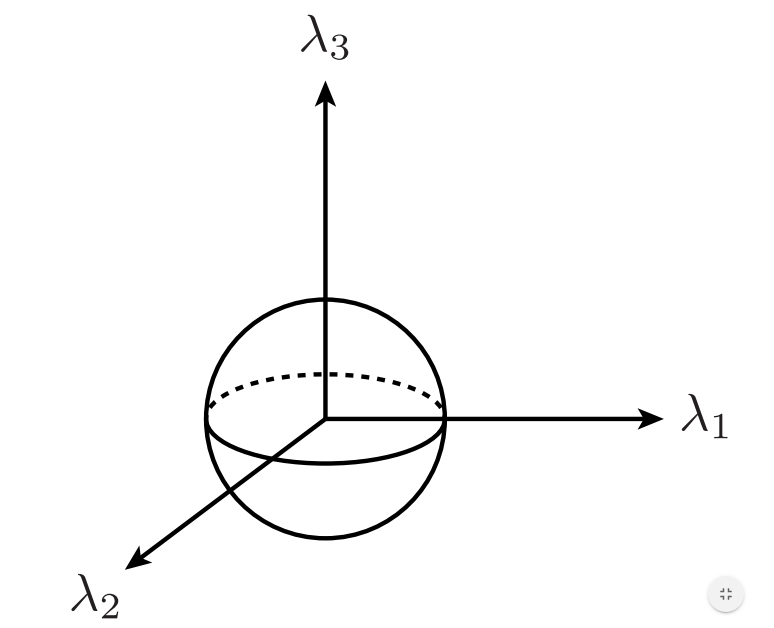
\includegraphics[width=1.2cm]{imgs/blob.png} \\
\end{tabular}
\end{center}
Frangiho filtr je vhodné použít opakovaně v různých měřítkách a různém natočení Hessovy matice v 3D obraze. Výsledky jednotlivých filtrací jsou pak zkombinovány celková míra důvěry ve skutečnost že se jedná o cévu je spočetena dle následujícího vztahu:
 \begin{equation}
\hat{V}(x) = \max_{s_{min}\leq s\leq s_{max}} v(x,s)
\end{equation}
\end{document}